\documentclass[conference]{IEEEtran}
\IEEEoverridecommandlockouts
% The preceding line is only needed to identify funding in the first footnote. If that is unneeded, please comment it out.
\usepackage[noadjust]{cite}
\usepackage[utf8]{inputenc}
\usepackage[T1]{fontenc}
\usepackage[ngerman]{babel}
\usepackage{cite}
\usepackage{amsmath,amssymb,amsfonts}
\usepackage{algorithmic}
\usepackage{graphicx}
\usepackage{float}
\usepackage{textcomp}
\usepackage{multicol}
\usepackage[colorinlistoftodos,prependcaption,textsize=tiny]{todonotes}
\def\BibTeX{{\rm B\kern-.05em{\sc i\kern-.025em b}\kern-.08em
    T\kern-.1667em\lower.7ex\hbox{E}\kern-.125emX}}

%override ieee citation style
\renewcommand{\citepunct}{,\penalty\citepunctpenalty\,}
\renewcommand{\citedash}{--}% optionally
\begin{document}

\selectlanguage{ngerman}
\title{Einschätzung der Fahrtauglichkeit eines Fahrers mit Wearables oder Smartphone}

\author{\IEEEauthorblockN{Niklas Kiefer}
\IEEEauthorblockA{\textit{Hochschule Harz} \\
Wernigerode, Deutschland \\
u33505@hs-harz.de}}

\maketitle

\begin{abstract}

\end{abstract}

\begin{IEEEkeywords}
evaluate fitness to drive, smartphones, smartwatches, smarttracking
\end{IEEEkeywords}

\section{Introduction}
This document is a model and instructions for \LaTeX.
Please observe the conference page limits. 
\section{Hintergrund und Related Works}
\label{relatedWork}
Dieser Abschnitt beschäftigt sich mit der Aufbereitung artverwandter Arbeiten zum Thema Einschätzung der Fahrtauglichkeit. Zuerst wird ein Überblick über gängige Richtlinien in der Verkehrspsychologie gegeben. Anschließend wird eine kurze Übersicht über bereits entwickelter Software, schwerpunktmäßig mobile Apps, in diesem Bereich aufgeführt. 

\subsection{Richtlinien zur Fahrtauglichkeit} 

Grundlage für den Begriff der Fahrtauglichkeit sind in der Bundesrepublik Deutschland \S 11 und \S 12 FeV\footnote{\label{foot:fev}Verordnung über die Zulassung von Personen zum Straßenverkehr (Fahrerlaubnis-Verordnung - FeV)} sowie Anhang III der aktuellen Führerscheinrichtlinie 2006/126/EG in der EU. In beiden Verordnungen werden jeweils körperliche sowie geistliche Eigenschaften des Fahrers zur Einschätzung gefordert. Ein besonderes Maß erhält die Beurteilung der Sehfähigkeit. Nachfolgend genannte Richtlinien haben die beiden Verordnungen als Grundlage.

Die Begutachtungsleitlinien zur Kraftfahreignung der Bundesanstalt für Straßenwesen dienen der differenzierten Einschätzung der Fahrtauglichkeit \cite{begutachtungsrichtlinien}. Sie geben einen Überblick über notwendige körperliche und geistige Fähigkeiten eines Fahrers im Straßenverkehr.
Auf Grundlage dessen beschäftigt sich die Arbeit von Poschadel und Falkenstein mit einer Reihe von Tests zur psychologischen Fahreinschätzung \cite{testverfahrenpsychometrischefahreignung}. Viel wesentlicher ist in dieser Arbeit aber die Evaluation der vorher in den Begutachtungsleitlinien zur Kraftfahreignung aufgeführten "Testgütekriterien" \cite{begutachtungsrichtlinien}. Als weitere Arbeit in diesem Kontext sind die Beurteilungskriterien von Schubert et al. zu nennen \cite{beurteilungskriterien}. Stellvertretend für die Deutsche Gesellschaft für Verkehrspsychologie werden eine Reihe von Kriterien für einen psychologischen Test zur Fahrtauglichkeit genannt. Vermehrt wird jedoch auf das Fahren unter Alkohol - und Drogeneinfluss, sowie auf vergangene Verkehrsauffälligkeiten des zu Testenden bezogen. Allgemeine, persönliche Eigenschaften finden nur einen kleinen Teil in dieser Richtlinie. 

Die Richtlinie der Driver \& Vehicle Licensing Agency ist der Standard der Fahrtauglichskeitseinschätzung im britischen Raum \cite{drivervehiclelicencingagency}. In ihr werden eine Reihe von Anforderungen an einen Fahrer aufgeführt, sowie verschiedene psychische und körperliche Krankheiten sowie deren Einfluss in der Einschätzung der Fahrtauglichkeit.

Die aufgeführten Richtlinien dienen als Ausgangspositionen bei der Ermittlung praxistauglicher Evaluationsparameter für diese Arbeit. Sie dienen außerdem als Grundlage für weitere Arbeiten in der Verkehrspsychologie, auf die zum Teil noch in Kapitel \ref{parameters} verwiesen wird.

\subsection{Softwaretechnische Ansätze}

Bereits in mehreren wissenschaftlichen Arbeiten wurde verschiedene Software beschrieben, die sich mit einzelnen Aspekten der Fahrtauglichkeit beschäftigen. Zum Beispiel haben Albrecht et al. in ihrer Arbeit eine App entwickelt, die einen Nystagmus\footnote{\label{foot:nystagmus} Nystagmus: unkontrollierbare, rhythmisch verlaufende Bewegungen eines Organs, am häufigsten die des Auges}  der Augen über einen Eye-Tracking-Kameratest ermitteln kann \cite{mobilesmarttracking}. Damit könne man einen starken Alkoholkonsum, sowie die Einnahme von Betäubungsmitteln durch den Fahrer nachweisen.

Ein ähnliche Herangehensweise hatte bereits Khosravianarab in seiner Arbeit zur Erstellung eines mobilen Testsystems zur Überprüfung auf Trunkenheit \cite{sobrietymobiletests}. Smartphones sollen dabei verwendet werden, um polizeilichen Einsatzkräften in einer Kontrolle eine schnelle und genaue Ermittlung von Alkohol - oder Drogenkonsum eines Fahrers zu ermöglichen. Hierbei wird wiederum der Nystagmus der Augen durch etwaige Eye-Tracking-Kameratests über das Smartphone ermittelt.

Nefzger hat in seiner Arbeit zu der Software \textit{Sensor Platform} ein Konzept für eine kostengünstige Plattform zur Bewertung des Fahrverhaltens mithilfe von Fahrerassistenzsystemen, vorrangig mit Sensoren des Smartphones herausgearbeitet \cite{smartphoneresearchplatform}. Die Nutzung von Smartphones anstatt professioneller Fahrerassistenzsysteme wäre demzufolge finanziell attraktiver, die Datenqualität wäre jedoch deutlich schlechter.

Die Analyse des Fahrverhaltens war ebenfalls Schwerpunkt in der Arbeit von Bo, Jian und Li zur Software \textit{Texive} \cite{texive}. Sie beschäftigen sich sehr detailliert mit der Erkennung, ob ein Fahrer während der Fahrt Textnachrichten mit dem Smartphone schreibt. Hierfür werden die Sensoren des Smartphones genutzt, um festzustellen, ob sich ein Fahrer auf dem Weg zur Fahrertür bewegt, er sich bereits im Auto befindet, oder das Auto sich gerade bewegt.

Weiter haben Bergasa et al. in ihrer Entwicklung zur App \textit{DriveSafe} eine Technology aufgeführt, die nur mithilfe der Sensoren von Smartphones das Fahrverhalten eines Fahrers überprüfen können \cite{drivesafe}. Dabei wird ein Punktesystem vorgestellt, womit das Smartphone Fahrablenkungen oder Stress beim Fahrer erkennt.

Einen Weg, psychische Messparameter in Bewertungen mittels aktueller Technologie einfließen zu lassen, zeigen Campos et al. in ihrer Arbeit auf \cite{drivingsimulations}. Sie beschreiben, wie auf Grundlage von psychologischen Tests Fahrszenarios im Fahrsimulator generiert werden, um die Fahrtauglichkeit des Fahrers in solchen Situationen zu testen. Einen ähnlichen Ansatz verfolgen Hirsekorn und Taylar, in dem sie Virtual Reality Anwendung nutzen, um Fahrer in bestimmten Fahrsituationen einschätzen zu können \cite{vrapplications}.

Der Schwerpunkt vieler verwandter Arbeiten lag in der Messung einzelner Parameter, wie zum Beispiel dem Alkoholismus \cite{mobilesmarttracking,sobrietymobiletests} sowie dem Verhalten des Fahrers während der Fahrt \cite{smartphoneresearchplatform, texive, drivesafe}. Andere Beiträge beschäftigen sich wiederum mit Technologien, die nicht ohne weiteres am Fahrzeug anzubringen sind, wie zum Beispiel die Fahrsimulation \cite{drivingsimulations, interaktivefahrsimulation, vrapplications}. Der Einsatz von bewährten psychologischen Tests fand nur wenig Anwendung. Diese Arbeit soll nun eine Möglichkeit aufzeigen, verschiedene gewählte Parameter \textit{vor dem Fahrtantritt} mit verschiedenen Techniken, Sensoren und appgestützten Fahrertests zu messen und gebündelt auszuwerten.

\section{Feststellung geeigneter Parameter}
\label{parameters}

Diese Arbeit soll sich im großen Maße mit der Ermittlung geeigneter Parameter für die Einschätzung der Fahrtauglichkeit beschäftigen. Dazu werden im Folgenden verschiedene Parameter aus im Abschnitt \ref{relatedWork} genannten Richtlinien genannt und erläutert. Im nächsten Schritt werden dann Möglichkeiten der Messung dieser Parameter aufgeführt. Daraus wird dann eine Auswahl von gut messbaren Parametern getroffen, auf welche sich dann in den folgenden Teilen dieser Arbeit stärker bezogen wird.
\subsection{Ermittlung der Parameter}

Die Richtlinie der Driver \& Vehicle Licensing Agency \cite{drivervehiclelicencingagency} führt bereits ein detaillierten Überblick von zu bewertenden Parametern auf:

\begin{multicols}{2}
\begin{itemize}
	\item Sehvermögen
	\item Visuelle Raumvorstellung
	\item Hörvermögen
	\item Aufmerksamkeit und Konzentration
	\item Gedächtnis
	\item Einsicht und Verständnis
	\item Urteilsfähigkeit
	\item Reaktionsfähigkeit
	\item Persönliche Organisation
	\item Selbstkontrolle
	\item Sensitivität
	\item Körperliche Voraussetzungen
	\item Koordination
	\item Adaptive Strategien (Anpassungsfähigkeit)
\end{itemize}
\end{multicols}

Bei den Körperlichen Voraussetzung wird hierbei speziell auf die Muskelkraft und - kontrolle verwiesen. Die Begutachtungsleitlinien zur Kraftfahreignung \cite{begutachtungsrichtlinien} und die daraus abgeleiteten unterstützenden Testverfahren \cite{testverfahrenpsychometrischefahreignung} folgen im wesentlichen diesen Parametern, zählen aber die Belastbarkeit und den Stress bzw. Aggression des Fahrers als wichtige Kriterien hinzu. Beide Richtlinien beziehen sich auch vermehrt auf psychische Fahrereigenschaften, zu körperlichen Eigenschaften zählen sie eher Bewegungsbehinderungen und körperliche Erkrankungen. Weitere mögliche Parameter zur Einschätzung der Fahrtauglichkeit können nach Schubert et al. \cite{beurteilungskriterien} erhöhter Alkohol - bzw. Drogenkonsum, sowie der Vergleich der Strafakte auf vorhergehende Auffälligkeiten im Straßenverkehr sein. Zumindest zweites ist vermutlich datenschutzrechtlich bedenklich.

\subsection{Möglichkeit der Messungen}
Eine Vielzahl der gefundenen Parameter lässt sich sehr gut durch Psychologische Tests untersuchen. Diese haben sich in der Praxis bewehrt und könnten auf dem Smartphone eingesetzt werden, indem der Fahrer vor Fahrtantritt eine Reihe solcher Tests absolvieren muss, bevor das Fahrzeug in Bewegung gesetzt werden darf. Poschadel und Falkenstein \cite{testverfahrenpsychometrischefahreignung} heben besonders das \textit{Wiener Testsystem} im Einsatz innerhalb der Verkehrspsychologie heraus. Dieses wird von der Firma \textit{SCHUHFRIED GmbH} entwickelt, und listet insgesamt 113 Einzeltests\footnote{\label{foot:schuhfriedtests} Schuhfried.at. (2018). SCHUHFRIED - Alle Tests. [online] Verfügbar unter: https://www.schuhfried.at/tests/alle-tests/ [Zugriff 28 Jan. 2018].} in verschiedenen Ausführungen zur Überprüfung psychischer Eigenschaften. Beispielsweise sieht man in der Abbildung \ref{fig:atavt} den Adaptiven Tachistoskopischen Verkehrsauffassungstest (ATAVT), der die Anpassungs - und Beobachtungsfähigkeit eines Fahrers im Straßenverkehr testet. Des weiteren bietet der Entwickler eine Schnittstelleninteraktion der Testsysteme an, um diese in neue Softwaresysteme einzubetten. Somit wäre eine Integration der Tests in mobilen Apps denkbar.

\begin{figure}[H]
\centering
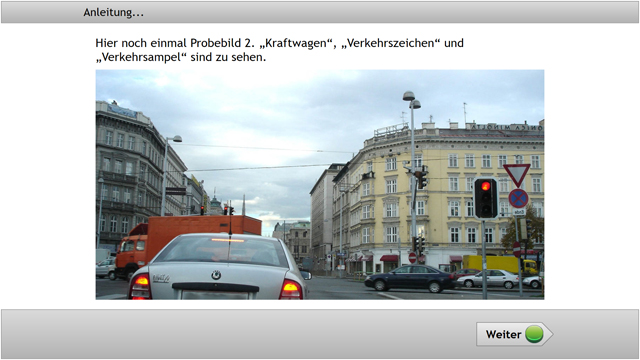
\includegraphics[width=0.95\linewidth]{images/atavt}
\caption[Caption for parameters]{Adaptiver Tachistoskopischer Verkehrsauffassungstest zur Überprüfung der Anpassungs - und Beobachtungsfähigkeit im Straßenverkehr \footnotemark}
\label{fig:atavt}
\end{figure}
\footnotetext{\label{foot:atavt} Schuhfried.at. (2018). SCHUHFRIED - ATAVT. [online] Verfügbar unter: https://www.schuhfried.at/test/ATAVT [Zugriff 1 Feb. 2018].}

Des Weiteren zeigen Studien zum Thema kognitiver Tests in der Verkehrspsychologie, wie u.a. von Bennett et al. \cite{cognitivetestsfitnesstodrive}, dass oft eine Reihe verschiedener Tests nötig ist, um ein valides Bild der Fahrtauglichkeit zu gewinnen. Über die Qualität einzelner Tests wird im Abschnitt \ref{dataValidity} noch mithilfe von Studien diskutiert \cite{cognitivetestsfitnesstodrive, reviewofassessmenttests, studieaufmerksamkeitstests, indiaassessment}.

Schwierig wird nun das Vorhaben, die genannten Tests auf dem Smartphone in App-Tests abzubilden. Diese Umsetzbarkeit wird nachfolgend im Abschnitt \ref{dataValidity} beurteilt.

Weitere Möglichkeiten der Messung bieten Wearables. Die in ihnen eingebauten Sensoren können Teile der vorher genannten Parameter direkt oder indirekt überprüfen. Tatsächlich hat die Recherche ergeben, dass Wearables bislang selten direkten Einsatz in der Verkehrspsychologie erhalten haben. Jedoch ist eines der Haupteinsatzfelder, Körperfunktionen, wie zum Beispiel die Herzfrequenz, zu messen und entsprechend auszuwerten. Diese Messfunktionen einigen sich sehr gut, um die körperlichen Voraussetzungen des Fahrers vor Fahrtantritt gezielt auszuwerten. Beispielsweise zählen Patel et al. die Möglichkeiten von Wearables mit der Messung von Herzfrequenz, Atemfrequenz, Blutdruck, Blutsauerstoffsättigung und Muskelaktivität sehr hoch ein \cite{reviewwearablesensors}. Viele der in ihrer Arbeit genannten Sensoren sind in gängigen Smartwatches und Fitness-Armbändern jedoch nicht eingebaut. Vielmehr bewerten  El-Amrawy et al. das Potenzial mit der Messung von Fitnessaktivität (über Schrittzähler), Puls, Gewicht, Herzfrequenz, Sauerstoffgehalt im Blut und Schlafmuster etwas geringer \cite{wearabletracking}. Trotzdem lassen sich damit bereits eine Menge von körperlichen Parametern bezüglich der Fahrtauglichkeit einschätzen. Interessant bleibt zu betrachten, wie präzise und glaubwürdig diese Einschätzung ist. Dies wird im Abschnitt \ref{dataValidity} noch untersucht.

Aus den gewonnen Erkenntnissen der Recherche zu psychologischen und kognitiven Tests zur Fahreignung, sowie aus den erarbeiteten Möglichkeiten zur Ermittlung einzelner Parameter mittels mobilen Sensoren, lässt sich sehr gut eine zweigeteilte Aufteilung der gewählten Parameter erstellen. Dies teilt sich zum einen in die Parameter, die sich mithilfe bewährter psychologischer Tests mittels Smartphone-App überprüfen lassen. Diese werden in der Tabelle \ref{tab:ps} mit zugehöriger Messmethode dargestellt. Das Kürzel dient zur besseren Referenzierung in den folgenden Kapiteln. 

\begin{table}[htbp]
	\caption{Übersicht gewählter Parameter in Messkategorie \textit{App-Tests Smartphone} (PS)}
	\begin{center}
		\begin{tabular}{c c c }
			\hline
			Kürzel& \textbf{Parameter} & \textbf{\textit{Möglichkeit der Messung}}\\
			\hline
			PS01 & Aufmerksamkeit \& Konzentration& Cognitrone-Test (COG)  \\
			PS02 & Sehvermögen& Test nach Albrecht et al. \cite{mobilesmarttracking}, \\
			&& teilweise Linienverfolgungstest (LVT) \\
			PS03 &Visuelle Raumvorstellung&Adaptiver Dreidimensionaler \\
			&&Würfeltest (A3DW), \\ 
			&&Intelligenz-Basis-Funktionen-\\
			&&Test (IBF) \\
			PS04 & Gedächtnis& Visueller Gedächtnistest (VISGED)\\
			PS05 & Belastbarkeit & Wiener Determinationstest (DT) \\
			PS06 & Anpassungsfähigkeit & Adaptiver Tachistoskopischer \\
			&&Verkehrsauffassungstest (ATAVT) \\
			PS07&Reaktionsfähigkeit&Wiener Reaktionstest (RT) \\
			&& Trail-Making-Test (TMT) \\
			PS08&Selbstkontrolle&IVPE-R-Test \\
			PS09&Persönliche Organisation&Tower of London-Test (TOL-F) \\
			PS10&Alkoholauffälligkeit&Fragebogen zum funktionalen \\
			&&Trinken (FFT), Test \\
			&&nach Albrecht et al. \cite{mobilesmarttracking} \\
			PS11&Aggression&Verkehrsspezifischer Itempool (VIP) \\
			\hline
		\end{tabular}
		\label{tab:ps}
	\end{center}
\end{table}

Die zweite Kategorie umfasst alle die Parameter, die sich mithilfe von Wearables messen lassen. Diese werden in der nachfolgenden Tabelle \ref{tab:pw} dargestellt und erhalten wiederum ein Kürzel zur späteren Referenzierung.

\begin{table}[htbp]
	\caption{Übersicht gewählter Parameter in Messkategorie \textit{Smart-Tracking Wearables} (PW)}
	\begin{center}
		\begin{tabular}{c c c }
			\hline
			Kürzel& \textbf{Parameter} & \textbf{\textit{Möglichkeit der Messung}}\\
			\hline
			PW01 & Körperliche Fitness & Aktivitäts - und  \\
			&& Blutsauerstoffsättigungsmessung \\
			&& (Wearable) \\
			PW02 & Koordination & Gyroskop - und \\
			&& Gleichgewichtssensor (Wearable) \\
			PW03 & Stressliche Belastung & Puls - und \\
			&& Herzfrequenzmessung \\
			&& (Wearable) \\
			PW04 & Müdigkeit & (indirekt) Schlafanalyse \\
			&& (Wearable) \\
			\hline
		\end{tabular}
		\label{tab:pw}
	\end{center}
\end{table}
\section{Analyse der Datenvalidität}
\label{dataValidity}
Nachdem im Abschnitt \ref{parameters} eine Reihe von geeigneten Parametern ermittelt wurde, soll die Qualität der aus den darauf beruhenden Messmöglichkeiten untersucht werden.

\subsection{Kategorie App-Tests Smartphone (PS)}

Die einzelnen Parameter werden im folgenden nacheinander mithilfe verschiedener Quellen auf Qualität überprüft. Auf die Aufgabenstellung einzelner Tests wird in dieser Arbeit nicht eingegangen. Die SCHUHFRIED GmbH verweist auf den einzelnen Unterseiten der im folgenden genannten Tests, dass sie Rasch-Modell-konform seien. Damit ist gemeint, dass die Testergebnisse ``spezifisch objektive, d.h. item- und personenunabhängige Testresultate" \footnote{Spektrum.de. (2018). Rasch-Modell - Lexikon der Psychologie. [online] Verfügbar unter: http://www.spektrum.de/lexikon/psychologie/rasch-modell/12443 [Zugriff 4 Feb. 2018].} erzielen. Dies sei ein sehr wichtiges Kriterium, um die Validität von derartigen, psychologischen Tests zu bewerten.

Laut der Studie von Kramm ist der 1992 entwickelte Cognitrone-Test (\textit{PS01}) zuverlässig in der Bestimmung der Aufmerksamkeit - und Konzentrationsleistung \cite{studieaufmerksamkeitstests}. Die Studie von Neelima schätzt die Vertrauenswürdigkeit der Testergebnisse eher durchschnittlich ein \cite{indiaassessment}. Mit einer Dauer von ca. 6-10 Minuten sei er zudem relativ kurz. Die Schwierigkeit des Tests sei mit zunehmenden Alter jedoch als sehr hoch einzuschätzen. In Hinsicht zur Situation des Fahrers, dass etwaige Tests schnell vor dem Fahrtantritt bewältigt werden müssen, ist eine kurze Testdauer und eine ausgewogene Schwierigkeit essentiell. Dieses Problem wird im Abschnitt \ref{openChallenges} noch thematisiert.

Parameter \textit{PS02} kann u.a. mit dem vom Albrecht et al. entwickelten System untersucht werden \cite{mobilesmarttracking}. Hier sei es möglich, mithilfe der Kamera eines Smartphones einen Nystagmus des Auges festzustellen. Die Ergebnisse seien sehr vielversprechend. Durch soll ein Augenzittern ist ein verminderndes Sehvermögen des Fahrers durchaus beurteilbar. Anderseits beschreiben Albrecht et al. ebenfalls, dass das aufgezeigte System als Teil einer umfänglicheren Testbatterie, und nicht als einziges Indiz genutzt werden sollte \cite{mobilesmarttracking}. Als weitere Testmaßnahme zum Sehvermögen kann indirekt der Linienverfolgungstest gewählt werden. Eine schlechte Sehleistung könnte bei diesem dazu führen, dass Linienverläufe falsch erkannt werden. Somit könnte man durch ein schlechtes Testergebnis auf eine schlechte Sehleistung folgen. Die Ermittlung des Sehvermögens bleibt jedoch kritisch in diesem Kontext. Zwar gibt es indirekte Methoden zur Bestimmung, jedoch führt selbst die Wiener Testreihe keinen eindeutigen Test zur direkten Messung.

Das räumliche Vorstellungsvermögen (\textit{PS03}) könnte mit dem Adaptiven Dreidimensionalen Würfeltest getestet werden. Laut der Studie von Bennett et al. hat der Test auch eine gute Zuverlässigkeit \cite{cognitivetestsfitnesstodrive}. Jedoch hat der Test eine Länge zwischen 29 und 52 Minuten\footnote{Schuhfried.at. (2018). SCHUHFRIED - A3DW. [online] Verfügbar unter: https://www.schuhfried.at/test/A3DW [Zugriff 1 Feb. 2018]} und wäre in dieser Form nicht einsetzbar. Der Intelligenz-Basis-Funktionen-Test prüft die räumliche Vorstellungskraft ebenfalls indirekt über einzelne Items. Somit kommt es auf die einzelnen Fragen innerhalb dieses Test an, um gezielt den Parameter PS03 zu überprüfen. Jedoch fassen Bennett et al. in ihrer Studie die Aussagekraft eines solchen Intelligenztest als nicht so hoch ein \cite{cognitivetestsfitnesstodrive}. PS03 ist somit mit genannten Test-Methoden eher nicht valide und wieder indirekt zu überprüfen.

Parameter \textit{PS04} kann mithilfe des Visuellen Gedächtnistests überprüft werden. In ähnlichen Ausführungen, wie z.B. dem Salford Objective Recognition Test, wird ein solcher Test in der Arbeit von Bennett et al. als vertrauenswürdig eingeschätzt \cite{cognitivetestsfitnesstodrive}.

Die Belastbarkeit (\textit{PS05})  kann unter anderem mit dem Wiener Determinationstest überprüft werden. Die Studie von Neelima schätzt die Validtät der Testergebnisse des DT auf gut bis durchschnittlich ein \cite{indiaassessment}. Schuhfried et al. haben eine umfassende Evaluierung dieses Tests vorgenommen und dessen Validität sehr detailliert bestätigt \cite{wiendt}. Der Test habe in seiner Kurform nur eine Dauer von 5 Minuten und keine hohe Komplexität, sei aber trotzdem sehr zuverlässig in der Messung der Belastbarkeit.

Der Parameter \textit{PS06} schließt neben der Anpassungsfähigkeit die verkehrstechnische Entscheidungsfähigkeit mit ein. Für beide Eigenschaften ist der ATAVT entwickelt wurden, um Situationen im Straßenverkehr zu präsentieren und die Beobachtungsfähigkeit des Fahrers einzuschätzen. Die Länge des Tests ist auf mindestens 8 Minuten\textsuperscript{\ref{foot:atavt}}  einzuordnen und somit relativ lang, um vor Fahrtantritt eingesetzt zu werden. Zudem bewertet Neelima in ihrer Studie die Validität des ATAVT eher durchschnittlich \cite{indiaassessment}.

Der Trail-Making-Test  ist laut der Studie von Bennett et al. eines der international renommiertesten Tests für das Messen der Reaktionsfähigkeit (\textit{PS07}) \cite{cognitivetestsfitnesstodrive}. Ebenfalls haben Baker et al. festgestellt, dass dieser Test sehr häufig in anderen Studien benutzt  und zudem als sehr zuverlässig eingeschätzt wird \cite{reviewofassessmenttests}. Zudem dauert der Test nur wenige Minuten und wäre somit auf dem Smartphone sehr einfach implementierbar und vor Fahrtantritt schnell ausführbar. Der Wiener Reaktionstest ist eine weitere Möglichkeit, um die Reaktionsfähigkeit zu testen. Er ist mit 5-10 Minuten Testdauer\footnote{Schuhfried.at. (2018). SCHUHFRIED - RT. [online] Verfügbar unter: https://www.schuhfried.at/test/RT [Zugriff 1 Feb. 2018]} relativ kurz. Das einfache, schnelle Drücken von Farbpunkten auf dem Smartphone-Display wäre keine große Implementierungsaufgabe.

Zur Überprüfung der Fähigkeit zur Selbstkontrolle (\textit{PS08}) eines Fahrers werden gängigerweise Fragebögen wie der IVPE-Test (Inventar verkehrsrelevanter Persönlichkeitseigenschaften) genutzt. Das Problem an solchen Fragebögen haben Torner et al. in ihrer Arbeit herausgearbeitet \cite{verfalschbarkeitivpe}. Demnach seien Persönlichkeitstest wie der IVPE-Test leicht verfälschbar, da sie vom Fahrer selbst vorgenommen werden und zum Teil unehrliche Antworten gegeben werden. Außerdem sind solche Fragebogen durch ihre zunehmende Dauer schlecht einsetzbar vor dem Fahrtantritt.

Um die Fähigkeit zur persönlichen Organisation (\textit{PS09}) eines Fahrers zu testen, wird oft der psychologische Test 'Tower of London' gewählt. Nach der Studie von Kaller et al. kann das Bewältigen dieses Planungstests auf eine erhöhte Planungsfähigkeit hinweisen \cite{toweroflondon}. Der Test kann jedoch durch seine Schwierigkeit sehr lang dauern.

Mit dem Thema der Erkennung von Alkoholismus (\textit{PS10}) eines Fahrers haben sich gleich mehrere Arbeiten beschäftigt \cite{mobilesmarttracking,sobrietymobiletests}. Dieses Kriterium wurde zudem von gängigen Richtlinien als sehr wichtig eingestuft \cite{begutachtungsrichtlinien,testverfahrenpsychometrischefahreignung,beurteilungskriterien,drivervehiclelicencingagency}. Die von Albrecht et al. aufgezeigte Kamera-App hat gezeigt, dass es sehr gut möglich ist, einen Nystagmus des Auges zu erkennen und darauf auf einen alkoholisierten, und somit nicht fahrtauglichen Zustand des Fahrers zu schließen \cite{mobilesmarttracking}. Des weiteren gäbe es die Möglichkeit, durch Fragebogen den Umgang eines Fahrers mit Alkohol zu bestimmen, wie zum Beispiel dem Fragebogen zum funktionalen Trinken (FFT). Jedoch haben wie beim Parameter \textit{PS08} solche Fragebögen den Nachteil, als Selbsttest nicht objektiv genug zu sein.

Der letzte Parameter in dieser Kategorie beschäftigt sich mit der Aggression eines Fahrers (\textit{PS11}). Auch hier lassen sich viele Fragebögen einsetzen, wie zum Beispiel der Verkehrsspezifische Itempool (VIP), der nebenbei noch viele weitere verkehrsrelevante Eigenschaften testet und mit ca. 10 Minuten \footnote{Schuhfried.at. (2018). SCHUHFRIED - VIP. [online] Verfügbar unter: https://www.schuhfried.at/test/VIP [Zugriff 3 Feb. 2018]} noch im Rahmen ist. Auch hier stellt das beim Parameter \textit{PS08} und \textit{PS10} genannte Problem der Verfälschbarkeit eine wichtige Rolle.

Zusammenfassend hat die Analyse der ersten Kategorie folgende Parameter inklusive Testverfahren als praxistauglich eingeschätzt:

\begin{itemize}
	\setlength\itemsep{2pt}
	\item PS01: Cognitrone (COG) 
	\item PS04: Visueller Gedächtnistest (VISGED) 
	\item PS05: Wiener Determinationstest (DT) 
	\item PS07: Wiener Reaktionstest (RT), Trail-Making-Test (TMT) 
	\item PS09: Tower of London (TOL) 
	\item PS10: App-Test nach Albrecht et al. \cite{mobilesmarttracking} 
\end{itemize}

In Abstrichen könnte jedoch auch der Verkehrsspezifische Itempool (VIP) genutzt werden, da dieser viele verschiedene Parameter abdeckt. Bei allen genannten Testverfahren bleibt in einer weiteren praktischen Anwendung zu untersuchen, inwieweit sich diese anwenden lassen.

\subsection{Kategorie Smart-Tracking Wearables (PW)}

Ein großes Problem in der Evaluation der einzelnen Messsensoren an Wearables ist die Größe des Marktes an derartigen Produkten. Viele der im folgenden genannten Studien beziehen sich auf einzelne Geräte. Im Rahmen dieser Arbeit soll eine allgemeine Möglichkeitsabschätzung getätigt werden. Eine detaillierter Vergleich der einzelnen Geräte ist nicht Inhalt.

Die allgemeine körperliche Fitness eines Fahrers (\textit{PW01}) kann zum Beispiel über die tägliche Aktivität des Fahrers gemessen werden. In alles Wearables gibt es Schrittzähler, die daraus Aussagen über die körperliche Verfassung der Nutzers generieren können.  El-Amrawy et al. haben kleine Unterschiede in der Genauigkeit von insgesamt 17 getesteten Geräten bestimmt \cite{wearabletracking}. Die Genauigkeiten zur tatsächlichen Schrittzahl seien zwischen 99.1\% (MisFit Shine) und 79.8 \%(Samsung Gear 2) ermittelt wurden, was insgesamt auf eine sehr hohe Validität schließen lässt. Case et al. haben in ihrer Studie u.a. die Genauigkeit des Beschleunigungssensors und Pedometers von Wearables untersucht \cite{studyaccuracysmartphoneapplications}. Mit Ausnahme eines einzigen Gerätes sei die Qualität sehr hoch. Parameter \textit{PW01} lässt sich außerdem durch die Überprüfung der Sauerstoffsättigung im Blut analysieren. Hierbei haben Preejith et al. untersucht, dass sich diese durch einen Fingersensor gut bestimmen lässt \cite{spo2oxygen}. 

Eine weitere wichtige körperliche Eigenschaft eines Fahrers ist die Balance (\textit{PW02}). Diese könnte mittels Gyroskop, Accelerometer und Gleichgewichtssensor in Wearables gemessen werden. Jedoch haben Mancini und Horak in ihrer Arbeit offen gelegt, dass Gleichgewichtsstörungen nur indirekt mithilfe dieser Sensoren zu messen sind und zusätzliche Berechnungen nötig sind \cite{balancewearables}. Shany et al. haben in ihrer Arbeit zusammengefasst, dass da Potenzial von solchen Sensoren in Wearables durchaus sehr groß ist, um die Balance eines Nutzers zu bestimmen \cite{sensorbasedfalls}. Jedoch geben auch sie an, dass viele Berechnungen nötig sind, um den Parameter einwandfrei bestimmen zu können. Eine weitere sehr interessante Möglichkeit, die Balance und Koordination zu messen ist es, Smartglasses einzusetzen. Nach der Studie von Salisbury et al. hätte diese Einschätzung eine Genauigkeit von bis zu 95 \% im Vergleich zu gängigen Balancemessungen und sei somit sehr vertrauenswürdig \cite{smartglasses}.

Die stressliche Belastung bzw. Aufregung eines Fahrers vor Fahrtantritt (\textit{PW03}) kann mithilfe eines Puls - oder Herzfrequenzsensors, der bereits in vielen Wearables integriert ist, überprüft werden. Jo et al. haben beispielsweise bestätigt, dass die Qualität verschiedener Fitness-Armbänder im Bereich Herzfrequenzmessung auseinander geht \cite{biofeedbackwearables}. Einigen Modelle wiesen eine hohe Validität auf, andere nicht. Ähnliche Ergebnisse erzielte Dooley in ihrer Arbeit, nach der die Validität verschiedener Geräte sehr unterschiedlich ausfällt \cite{selfmonitoringheartrate}. El-Amrawy et al. haben jedoch in ihrer Arbeit herausgefunden, dass die Genauigkeit der Messungen zwischen 99.9\% (Apple Watch) und 92.8\% allgemein sehr hoch sei \cite{wearabletracking}. 

Mithilfe der Schlafüberwachung, die an vielen Fitness-Armbändern implementiert ist, kann indirekt der Parameter \textit{PW04} gemessen werden. Das Systematische Literaturreview von Evenson et al. hat herausgearbeitet, dass die Validität und Vertrauenswürdigkrit dieser Schlafüberwachung bei sehr vielen Geräten sehr hoch ist \cite{reviewconsumerwearables}.

Zusammenfassend hat die Recherche für diese Kategorie ergeben, dass alle Parameter durchaus gute Ergebnisse liefern, um die körperlichen Eigenschaften eines Fahrers vor Fahrtantritt zu prüfen. Der große Vorteil gegenüber der ersten Kategorie ist hier, dass die Daten in Echtzeit genutzt werden können und keine minutenlangen Tests absolviert werden müssen.

\section{Konzept zur Datenerfassung und - auswertung}
\label{concept}
Ein weiteres wichtiges Thema dieser Arbeit soll es sein, ein erstes Konzept zur automatischen Datenerfassung und - auswertung der nötigen Parameterdaten zu entwickeln. Dieses kann dann als Vorlage für einen Prototypen zur automatischen Einschätzung der Fahrtauglichkeit eines Fahrers vor Fahrtantritt dienen. Der grundlegende Entwurf ist in der Abbildung \ref{fig:conceptfmc} als FMC-Modell dargestellt.

\begin{figure}
	\centering
	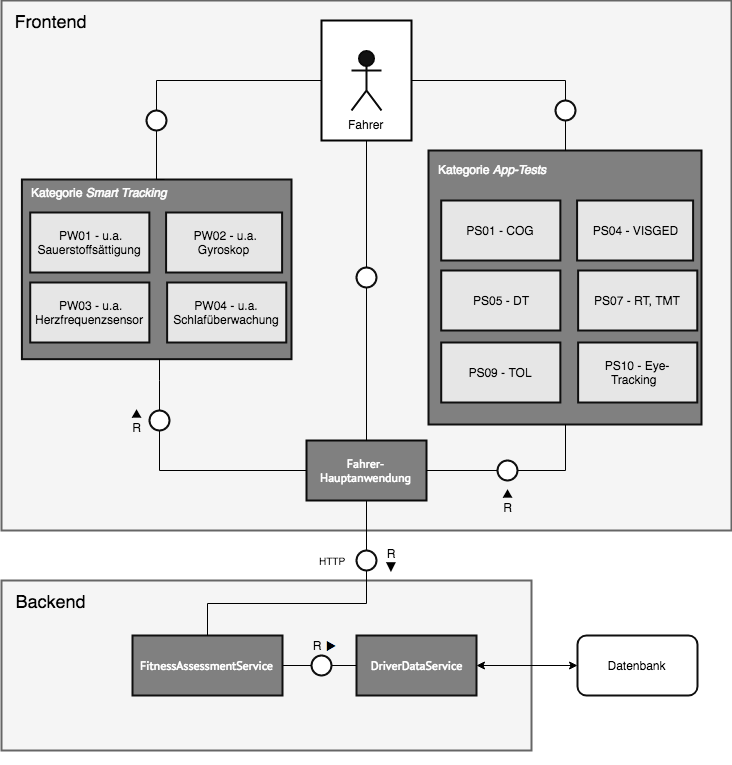
\includegraphics[width=\linewidth]{images/ConceptDriverAssessmentData}
	\caption[Caption for concept]{FMC-Modell der grundlegenden Anwendung}
	\label{fig:conceptfmc}
\end{figure}

Initiativ kann die Anwendung, zum Beispiel in Form einer Smartphone-App, manuell durch den Nutzer gestartet werden. Die Anwendung \textit{Texive} von Bo et al. hat jedoch auch gezeigt, dass automatisch erkannt werden kann, wenn sich der Fahrer im Fahrzeug befindet \cite{texive}. Ein denkbares Szenario wäre hier, dass die Lenkradsperre erst gelöst wird, wenn etwaige App-Tests (Kategorie App-Tests) auf dieser Anwendung erfolgreich absolviert werden. Dieses Szenario bringt jedoch Probleme mit sich, welche im Anschluss diskutiert werden. Realistischer wäre hierbei eher, dass die Hauptanwendung die körperlichen Fahrerdaten permanent aus gekoppelten  Wearables speichert und im Falle des Fahrtantritts auswertet. Abbildung \ref{fig:conceptfmc} zeigt hier die Vorgehensweise. Die Hauptanwendung als Teil des Frontends schickt die gebündelten Fahrerdaten aus beiden Parameter-Kategorien an das Backend. Es wird an dieser Stelle offen gelassen, ob die Auswertung der Daten auf dem Smartphone direkt oder auf einem separaten Server vorgenommen wird.

Idealerweise übernimmt dann ein eigenständiger Dienst, in Abbildung \ref{fig:conceptfmc} als \textit{FitnessAssessmentService} betitelt, die eigentliche Evaluation der Fahrerdaten. Für die Kategorie App-Tests werden hier die Test-Ergebnisse genommen. Eine hohe Punktzahl entspräche einer guten Fahrtauglichkeit. Bei der Kategorie Smart Tracking müsste noch evaluiert werden, inwieweit die einzelnen Parameter beim Fahrer ausgeprägt sein müssen, um Fahrtauglichkeit nachzuweisen. Die Anwendung \textit{DriveSafe} von Bergasa et al. hat ein Punktesystem vorgestellt, in welchem das Fahrverhalten bewertet wird \cite{drivesafe}. Aufbauend auf diesem könnte man eine ähnliche Bewertung der körperlichen Verfassung auf Grundlage der Fahrerdaten vornehmen. 

Denkbar wäre zudem, die Fahrerdaten dauerhaft zu persistieren. Somit können Zustandsmuster des Fahrers auf lange Sicht untersucht werden, um so ebenfalls Aussagen über die Verfassung des Fahrers zu treffen. Hilfreich wäre dies unter anderem bei Parameter \textit{PW04}, um eine auffällige Müdigkeit des Fahrers zu erkennen. Außerdem könnte für \textit{PW01} eine dauerhaft schlechte körperliche Verfassung erfasst werden. Die Persistenz-Vorgänge sollten dann über einen weiteren Dienst im Backend vorgenommen werden, auf welchem der \textit{FitnessAssessmentService} zugreifen könnte, um die nötigen Fahrerdaten dauerhaft zu erhalten. Dieser wird in Abbildung \ref{fig:conceptfmc} als \textit{DriverDataService} gekennzeichnet.

Letztendlich sendet der \textit{FitnessAssessmentService} eine abschließende Einschätzung der Fahrtauglichkeit an die Hauptanwendung. Denkbar wäre hier wieder, dass nur bei positivem Ergebnis das Lenkrad des Fahrzeugs entsperrt wird. 

\section{Diskussion und Offene Fragestellungen}
\label{openChallenges}

Neben den in den vorhergehenden Kapiteln genannten Ergebnissen haben sich eine Reihe von Problemen herauskristallisiert. Aus diesen lassen sich weitere interessante Forschungsfragen in diesem Themenbereich formulieren, welche im Folgenden erläutert werden sollen.

Im Abschnitt \ref{concept} wurde ein Konzept für die automatisierte Evaluation der Fahrtauglichkeit vorgestellt. Problematisch wird die Anwendung dann, wenn man die Anwenderseite betrachtet. Die Aussage, dass ein Fahrer die Tests zu jeder Zeit freiwillig vornehmen wird, ist als sehr kritisch einzustufen. Es bleibt zu betrachten, wie hoch die Bereitschaft auf Seiten der Fahrer ist, dass aufgezeigte System einzusetzen. Abhilfe könnte hier eine Pflichteinrichtung des Systems im Fahrzeug sein. Denkbar wäre, dass das Fahrzeug erst in Betrieb genommen werden kann, wenn das System die Fahrtauglichkeit des Fahrers bestätigt. Dies wäre beispielsweise bei bereits alkoholauffälligen Fahrern denkbar, muss aber weiter untersucht werden. Ein weiterer Punkt ist die Qualität der Daten. Zwar wurden im Abschnitt \ref{dataValidity} die Parameter ausgefiltert, die leicht verfälschbar sind. Dennoch können unter Drucksituationen oder in Notsituationen falsche Testergebnisse in der Parameter-Kategorie App-Tests vorliegen. Weiterhin muss untersucht werden, wie kurz die genannten Tests sein dürfen, um vorm Fahrtantritt benutzt zu werden. Des weiteren kann eine hohe Schwierigkeit der Tests dazu führen, dass die Frustration eines Fahrers sehr hoch wird. 

Weiterhin ist der Datenschutz eine wichtige Fragestellung, die betrachtet werden sollte. Zum einen müssen psychologische Fahrerdaten und Testergebnisse vor Missbrauch geschützt werden \cite{beurteilungskriterienleipzig}. Ebenfalls muss diskutiert werden, wie die körperlichen Daten aus dem Smart Tracking privat bleiben \cite{securityprivacyfitnesstracking}. Das im Abschnitt \ref{concept} dargestellte Konzept muss dementsprechend erweitert werden.

Des weiteren hat die Analyse der Datenvalidität gezeigt, dass die Ergebnisse der Sensoren zur Einschätzung der körperlichen Eigenschaften sehr gut sind. Weiterhin muss aber konzipiert werden, auf welcher Grundlage die Einschätzung getätigt werden müssen. Ein Punktesystem wie in der Anwendung \textit{DriveSafe} ist denkbar \cite{drivesafe}. Hinzu können dann auch Daten aus Smartphone-Sensoren genommen werden. Beispielsweise kann der eingebaute Schrittzähler ebenfalls Aussagen über die körperliche Fitness des Fahrers treffen \cite{validationphysicalactivitytracking,bewegungserkennungsensoren}. In dieser Arbeit wurde die Evaluation nur auf Grundlage der Sensoren in Wearables vorgenommen.

Ebenfalls nicht Teil dieser Arbeit war ein detaillierter Vergleich der einzelnen Geräte. Die im Abschnitt \ref{dataValidity} dargestellten Studien beschäftigten sich teilweise mit einzelnen Modellen, in dieser Arbeit wurden diese Ergebnisse verallgemeinert, um generelle Aussagen über die Datenvalidität der Sensoren zu treffen. Sicherlich muss beachtet werden, welche Wearables in einem etwaigen Prototypen genutzt werden und wie zuverlässig die gewonnenen Daten im Einzelfall sind.

\section{Zusammenfassung}
\label{conclusion}
Zusammenfassend lässt sich ohne weiteres sagen, dass die Einschätzung der Fahrtauglichkeit eines Fahrers mithilfe von Smartphones und Wearables möglich ist. Die Ergebnisse dieser Arbeit haben gezeigt, das gerade vor Fahrtantritt eine Reihe von Parametern gemessen werden können. Es wurde gezeigt, dass sich eine Aufteilung der zu messenden Fahrereigenschaften in zwei Kategorien anbietet. Zum einen können psychische und kognitive Parameter mittels bewährter Testverfahren ermittelt werden. Diese können in Smartphone-Applikationen integriert werden, die ein Fahrer vor Fahrtantritt zu bewältigen hat. Hinzukommen diverse körperliche Eigenschaften, die permanent von Sensoren in Wearables gemessen werden können.

Eine Reihe von Parametern in beiden Bereichen wurde zusammengefasst und dessen Qualität auf Grundlage zahlreicher Studien überprüft. Die Ergebnisse sind sehr vielversprechend, jedoch geschahen viele Arbeiten nicht im direkten Bereich der Verkehrspsychologie. Eine nähere Betrachtung ist als sehr lohnenswert einzuschätzen.

Ebenfalls wurde ein Konzept für eine Anwendung dargestellt, die eine Fahrtauglichkeitseinschätzung automatisiert vornehmen kann. Dieses kann als Grundlage für einen praxistauglichen Prototypen dienen.

Als großes Problem ist die Verbindlichkeit der gezeigten Anwendung als Fahrerassistenzsystem aufgetreten. Hier bleibt weiterhin zu diskutieren, inwieweit Bereitschaft eines Fahrers besteht, die automatisierte Einschätzung der Fahrtauglichkeit freiwillig im Auto einzusetzen.

\todo[inline]{Literatur ordnen!}

\begin{thebibliography}{00}

\bibitem{begutachtungsrichtlinien} N. Gräcmann, und M. Albrecht, 'Begutachtungsleitlinien zur Kraftfahreignung', Mensch und Sicherheit Heft M 115, Bergisch Gladbach, 2017
\bibitem{testverfahrenpsychometrischefahreignung} S. Poschadel, und M. Falkenstein, 'Testverfahren zur psychometrischen Leistungsprüfung der Fahreignung', Mensch und Sicherheit Heft M 203, Bergisch Gladbach, 2009
\bibitem{beurteilungskriterien} W. Schubert, R. Mattern, und J. Brenner-Hartmann, 'Beurteilungskriterien: Urteilsbildung in der Medizinisch-Psychologischen Fahreignungsdiagnostik', Bonn, 2013
\bibitem{drivervehiclelicencingagency} Driver \& Vehicle Licensing Agency, 'Assessing fitness to drive - a guide for medical professionals', DVLA, Swansea, 2017
\bibitem{wearabletracking} F. El-Amrawy, und M. I. Nounou, 'Are Currently Available Wearable Devices for Activity Tracking and Heart Rate Monitoring Accurate, Precise, and Medically Beneficial?', Alexandria University, Alexandria, 2015
\bibitem{interaktivefahrsimulation} T. Wolbers, J. Küst, H. Karbe, J. Netz, und V. Hörnberg, 'Interaktive Fahrsimulation - ein neuer Weg zur Diagnose und Rehabilitation der Fahrtauglichkeit', Rehabilitation 2001, Stuttgart, 2001
\bibitem{mobilesmarttracking} U. Albrecht, K. Khosravianarab, K. Folta-Schoofs, J. Teske, J. Kanngießer, und U. von Jan, 'Mobile Smarttracking – Finding objective parameters for determining fitness to drive', Biomedical Engineering / Biomedizinische Technik, Berlin, 2013
\bibitem{sobrietymobiletests}K. Khosravianarab, 'Development of a Mobile Test Suite to Determine the Sobriety of Motorists.', Göteborg, 2013.
\bibitem{smartphoneresearchplatform} M. C. Nefzger, 'Design and Development of a Low-Cost Smartphone-Based Research Platform for Real-World Driving Studies', Ludwig-Maximilians-Universität, München, 2017
\bibitem{texive} C. Bo, X. Jian, und X.-Y. Li, 'TEXIVE: Detecting Drivers Using Personal Smart Phones
by Leveraging Inertial Sensors',  Illinois Institute of Technology, Chicago, 2013
\bibitem{drivesafe} L. M. Bergasa, D. Almería, J. Almazán, J. J. Yebes, und R. Arroyo, 'DriveSafe: An app for alerting inattentive drivers and scoring driving behaviors', 2014 IEEE Intelligent Vehicles Symposium Proceedings, Dearborn, 2014
\bibitem{drivingsimulations}J. L. Campos, M. Bédard, und S. Classen, 'Guiding Framework for Driver Assessment Using Driving Simulators', Frontiers in Psychology, Toronto, 2017
\bibitem{vrapplications}L. Hirsekorn, S. Taylar, 'VR technology applications in determining fitness to drive', Cyberpsychology and Behavior, 1 (4), S. 385-389, New Rochelle, 2009
\bibitem{cognitivetestsfitnesstodrive}J.M. Bennett, E. Chekaluk, und J. Batchelor,
'Cognitive Tests and Determining Fitness to Drive in Dementia: A Systematic Review'
Journal of the American Geriatrics Society, 64 (9), S. 1904-1917, Sydney, 2016
\bibitem{studieaufmerksamkeitstests} T. Kramm, 'Normierungsstudie einer Aufmerksamkeits- Testbatterie (Vigilanz, Signal- Detection und Cognitrone des Wiener Testsystems der Dr. G. Schuhfried Ges. m. b. H.)', Ruhr- Universität zu Bochum, Mönchengladbach, 2000
\bibitem{indiaassessment} C. Neelima, 'Study related to the Prediction of Driving in India Assessment of Driving Behaviour and Safe Driving Skills of Goods Vehicle Drivers in India', New Delhi, 2014. 
\bibitem{wiendt} G. Schuhfried, W. Neuwirth, und M. Benesch, 'Wiener Testsystem - Manual Determinationstest', Schuhfried GmbH, Mödling, 2012
\bibitem{reviewofassessmenttests}A. Baker, C. A. Unsworth, und N. A. Lannin,
'Determining fitness to drive: A systematic review of the methods and assessments used after mild traumatic brain injury', British Journal of Occupational Therapy, 78 (2), pp. 73-86, London, 2015
\bibitem{verfalschbarkeitivpe} F. Torner, M. Litzenberger, und B. Schützhofer, 'Zur Problematik der Verfälschbarkeit von psychologischdiagnostischen Persönlichkeitsverfahren im Rahmen der Verkehrspsychologischen Untersuchung (VPU) in Österreich', Universität Wien, 2007
\bibitem{toweroflondon} C. P. Kaller, J. M. Unterrainer, und C. Stahl, 'Assessing planning ability with the Tower of London task: Psychometric properties of a structurally balanced problem set', Psychological Assessment, 2012
\bibitem{reviewwearablesensors} S. Patel, H. Park, P. Bonato, L. Chan, and M. Rodgers, 'A review of wearable sensors and systems with application in rehabilitation', 2012 Journal of NeuroEngineering and Rehabilitation, 2012
\bibitem{beurteilungskriterienleipzig} W. Jacobshagen, und Johannes Jansen, 'Evaluationsansätze zum komplexen medizinisch-psychologischen Begutachtungs-system "Beurteilungskriterien".', Tagungsband, S. 25, Dresden, 2009
\bibitem{healthylifeactivityrecognition} M. D. Thang, S. W. Loke, und F. Liu, 'HealthyLife: an Activity Recognition System with Smartphone using Logic-Based Stream Reasoning',  La Trobe University, Bundoora, 2012
\bibitem{fitnesstrackingbajpaj}  A. Bajpai, V. Jilla, V. N. Tiwari, S. M. Venkatesan, und R. Narayanan, 'Quantifiable fitness tracking using wearable devices,' 2015 37th Annual International Conference of the IEEE Engineering in Medicine and Biology Society (EMBC), Mailand, 2015
\bibitem{monitoringstressheartrate} S. Mayya, V. Jilla, V. N. Tiwari, M. M. Nayak, und R. Narayanan, 'Continuous monitoring of stress on smartphone using heart rate variability', 2015 IEEE 15th International Conference on Bioinformatics and Bioengineering (BIBE), Belgrade, 2015
\bibitem{selfmonitoringheartrate} E. E. Dooley, 'Measuring the Validity of Self-monitoring Heart Rate and Activity Tracking Wearables', University of Texas, Austin, 2016
\bibitem{biofeedbackwearables} E. Jo, K. Lewis, D. Directo , M. J.  Kim, und B.A. Dolezal. 'Validation of Biofeedback Wearables for Photoplethysmographic Heart Rate Tracking', Journal of Sports Science \& Medicine, 2016
\bibitem{activityrecognition} J. R. Kwapisz, G. M. Weiss, und S. A. Moore, 'Activity Recognition using Cell Phone Accelerometers', Fordham University, New York, 2010
\bibitem{activityrecognition2} S. Dernbach, B. Das, N. C. Krishnan, B. L. Thomas, und D. J. Cook, 'Simple and Complex Activity Recognition through Smart Phones', 2012 Eighth International Conference on Intelligent Environments, Guanajuato, 2012
\bibitem{securityprivacyfitnesstracking} W. Zhou, und S. Piramuthu, 'Security/privacy of wearable fitness tracking IoT devices', 2014 9th Iberian Conference on Information Systems and Technologies (CISTI), Barcelona, 2014
\bibitem{validationphysicalactivitytracking} E. B. Hekler, M. P. Buman, und L. Grieco, 'Validation of Physical Activity Tracking via Android Smartphones Compared to ActiGraph Accelerometer: Laboratory-Based and Free-Living Validation Studies', JMIR mHealth and uHealth. 2015
\bibitem{bewegungserkennungsensoren} S. Milker, 'Bewegungserkennung mit Smartphones mittels deren Sensoren', Universität Koblenz-Landau, Koblenz, 2012
\bibitem{reviewconsumerwearables} K. R. Evenson, M. M. Goto, und R. D. Furberg, 'Systematic review of the validity and reliability of consumer-wearable activity trackers', The International Journal of Behavioral Nutrition and Physical Activity, 2015
\bibitem{studyaccuracysmartphoneapplications} M. A. Case, H. A. Burwick, K. G. Volpp, und M. S. Patel, 'Accuracy of smartphone applications and wearable devices for tracking physical activity data', JAMA Volume 313, 2015
\end{thebibliography}

\end{document}
